\documentclass[paper=letter,11pt]{scrartcl}

\KOMAoptions{headinclude=true, footinclude=false}
\KOMAoptions{DIV=14, BCOR=5mm}
\KOMAoptions{numbers=noendperiod}
\KOMAoptions{parskip=half}
\addtokomafont{disposition}{\rmfamily}
\addtokomafont{part}{\LARGE}
\addtokomafont{descriptionlabel}{\rmfamily}
%\setkomafont{pageheadfoot}{\normalsize\sffamily}
\setkomafont{pagehead}{\normalsize\rmfamily}
%\setkomafont{publishers}{\normalsize\rmfamily}
\setkomafont{caption}{\normalfont\small}
\setcapindent{0pt}
\deffootnote[1em]{1em}{1em}{\textsuperscript{\thefootnotemark}\ }


\usepackage{amsmath}
\usepackage[varg]{txfonts}
\usepackage[T1]{fontenc}
\usepackage{graphicx}
\usepackage{xcolor}
\usepackage[american]{babel}
% hyperref is needed in many places, so include it here
\usepackage{hyperref}

\usepackage{xspace}
\usepackage{multirow}
\usepackage{float}


\usepackage{braket}
\usepackage{bbm}
\usepackage{relsize}
\usepackage{tcolorbox}

\def\ketY{\ensuremath{\ket {\Psi}}}
\def\iGeV{\ensuremath{\textrm{GeV}^{-1}}}
%\def\mp{\ensuremath{m_{\textrm{proton}}}}
\def\rp{\ensuremath{r_{\textrm{proton}}}}
\def\me{\ensuremath{m_{\textrm{electron}}}}
\def\aG{\ensuremath{\alpha_G}}
\def\rAtom{\ensuremath{r_{\textrm{atom}}}}
\def\rNucl{\ensuremath{r_{\textrm{nucleus}}}}
\def\GN{\ensuremath{\textrm{G}_\textrm{N}}}
\def\ketX{\ensuremath{\ket{\vec{x}}}}
\def\ve{\ensuremath{\vec{\epsilon}}}


\def\ABCDMatrix{\ensuremath{\begin{pmatrix} A &  B  \\ C  & D \end{pmatrix}}}
\def\xyprime{\ensuremath{\begin{pmatrix} x' \\ y' \end{pmatrix}}}
\def\xyprimeT{\ensuremath{\begin{pmatrix} x' &  y' \end{pmatrix}}}
\def\xy{\ensuremath{\begin{pmatrix} x \\ y \end{pmatrix}}}
\def\xyT{\ensuremath{\begin{pmatrix} x & y \end{pmatrix}}}

\def\IMatrix{\ensuremath{\begin{pmatrix} 0 &  1  \\ -1  & 0 \end{pmatrix}}}
\def\IBoostMatrix{\ensuremath{\begin{pmatrix} 0 &  1  \\ 1  & 0 \end{pmatrix}}}
\def\JThree{\ensuremath{\begin{pmatrix}    0 & -i & 0  \\ i & 0  & 0 \\ 0 & 0 & 0 \end{pmatrix}}} 
\def\JTwo{\ensuremath{\begin{bmatrix}    0 & 0 & -i  \\ 0 & 0  & 0 \\ i & 0 & 0 \end{bmatrix}}}
\def\JOne{\ensuremath{\begin{bmatrix}    0 & 0 & 0  \\ 0 & 0  & -i \\ 0 & i & 0 \end{bmatrix}}}
\def\etamn{\ensuremath{\eta_{\mu\nu}}}
\def\Lmn{\ensuremath{\Lambda^\mu_\nu}}
\def\dmn{\ensuremath{\delta^\mu_\nu}}
\def\wmn{\ensuremath{\omega^\mu_\nu}}
\def\be{\begin{equation*}}
\def\ee{\end{equation*}}
\def\bea{\begin{eqnarray*}}
\def\eea{\end{eqnarray*}}
\def\bi{\begin{itemize}}
\def\ei{\end{itemize}}
\def\fmn{\ensuremath{F_{\mu\nu}}}
\def\fMN{\ensuremath{F^{\mu\nu}}}
\def\bc{\begin{center}}
\def\ec{\end{center}}
\def\nus{$\nu$s}

\def\adagger{\ensuremath{a_{p\sigma}^\dagger}}
\def\lineacross{\noindent\rule{\textwidth}{1pt}}

\newcommand{\multiline}[1] {
\begin{tabular} {|l}
#1
\end{tabular}
}

\newcommand{\multilineNoLine}[1] {
\begin{tabular} {l}
#1
\end{tabular}
}



\newcommand{\lineTwo}[2] {
\begin{tabular} {|l}
#1 \\
#2
\end{tabular}
}

\newcommand{\rmt}[1] {
\textrm{#1}
}


%
% Units
%
\def\m{\ensuremath{\rmt{m}}}
\def\GeV{\ensuremath{\rmt{GeV}}}
\def\pt{\ensuremath{p_\rmt{T}}}


\def\parity{\ensuremath{\mathcal{P}}}

\usepackage{cancel}
\usepackage{ mathrsfs }
\def\bigL{\ensuremath{\mathscr{L}}}

\usepackage{ dsfont }



\usepackage{fancyhdr}
\fancyhf{}


\lhead{\Large 33-444} % \hfill Introduction to Particle Physics \hfill Spring 2022}
\chead{\Large Introduction to Particle Physics} % \hfill Spring 2022}
\rhead{\Large Spring 2022} % \hfill Introduction to Particle Physics \hfill Spring 2022}

\begin{document}
\thispagestyle{fancy}

\begin{center}
{\huge \textbf{Soft Photon and Gluon Theorems}}
\end{center}

{\fontsize{14}{16}\selectfont

\underline{Lorentz Invariance and ``Soft Limits''}

Punch line that we've been building to in first part of this course.

Matrix element we would get by scattering external $\gamma$.
\be
M = \epsilon^\mu M_\mu
\ee
where $\epsilon^\mu$ is some linear combination of two photon polarization vector $\epsilon^1$ and $\epsilon^2$


M is Lorentz Invariant, under Lorentz transformation
\be
M \rightarrow \epsilon'^\mu M'_\mu
\ee
where $M'_\mu = {\Lambda_\mu}^\nu M_\nu$

However (here comes the major constraint) $\epsilon$ is not  a full 4-vector.  
Only has 2 components.

Under little group transformations (you will show in your H.W.)
\be
\epsilon \rightarrow \underbrace{c_1 \epsilon_1^\mu + c_2 \epsilon_2^\mu}_{\substack{\epsilon' \textrm{ can only be made} \\ \textrm{ of these pieces}}} + \underbrace{c_3 p^\mu}_{\substack{\textrm{Not valid} \\ \textrm{``Not in Hilbert Space''}}}
\ee


So, 
\bea
M=\epsilon^\mu M_\mu &\rightarrow& \left(c_1 \epsilon_1^\mu + c_2 \epsilon_2^\mu + c_3 p^\mu \right) M'_\mu \\
&=& \epsilon'^\mu M'_\mu + \underbrace{c_3 p^\mu M'_\mu}_{\textrm{Must go to 0}}
\eea

\underline{We will see, this has enormous implications !!!}


Will be considering diagrams with external ``$\gamma$''s (mass-less spin 1 particles)

\begin{minipage}{0.4\textwidth}
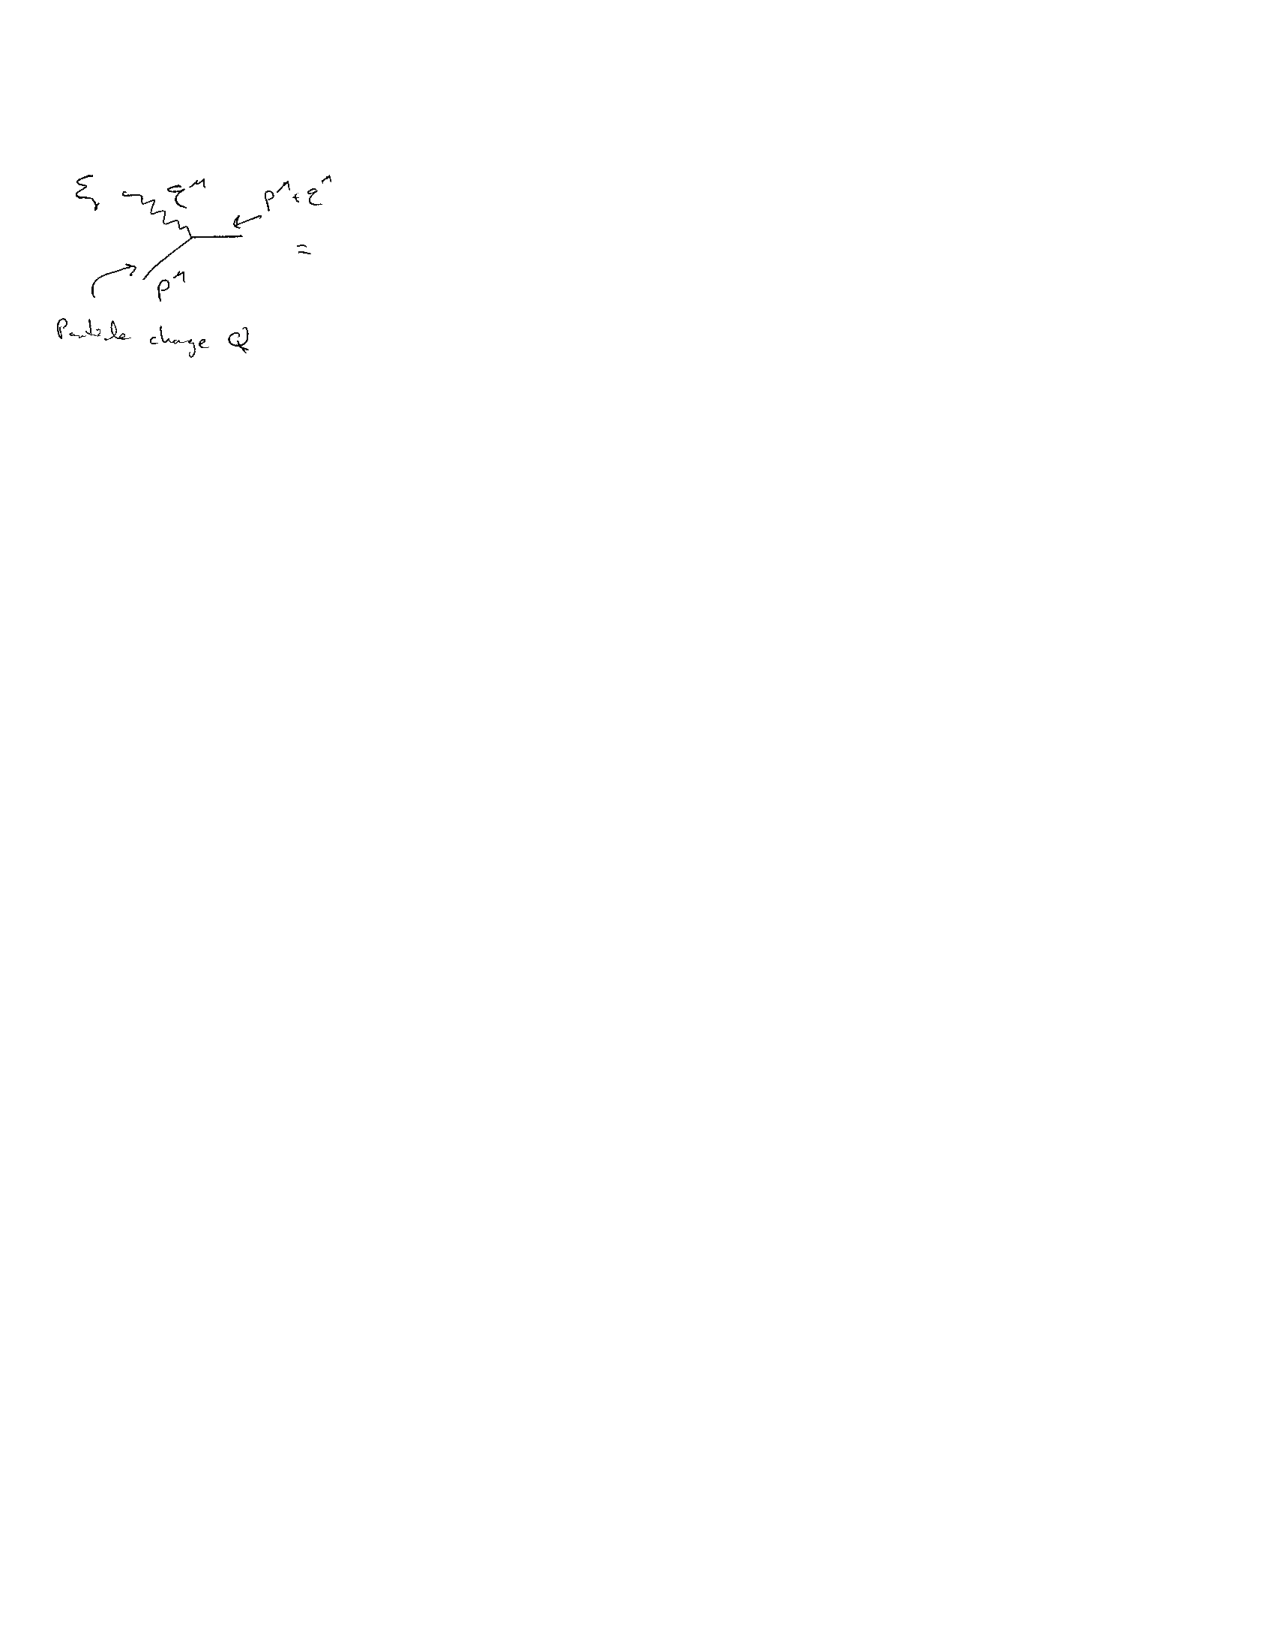
\includegraphics[width=0.9\textwidth]{./gammaVertex.pdf}
\end{minipage} %\hfill
\begin{minipage}{0.45\textwidth}
\bea
&=& iQ(p^\mu + (p^\mu + q^\mu)) \epsilon_\mu    \hspace*{1in} (q^\mu\epsilon_\mu = 0) \\
&=& iQ 2 p^\mu \epsilon_\mu
\eea
\end{minipage}

This is the most general form in the ``soft limit''  $q\rightarrow0$

\fbox{\begin{minipage}{0.6\textwidth}
\be
\Gamma_\mu \sim p_\mu F(q^2, p^2, p\cdot q) 
\ee
By dimensional analysis $F(q^2, p^2, p\cdot q) \rightarrow F(\frac{p\cdot q}{m^2})$
\end{minipage}}

\lineacross

Consider ``Compton Scattering''

Start with one type of spin-1 boson and one type of matter particle.

The diagram: 

\begin{minipage}{0.4\textwidth}
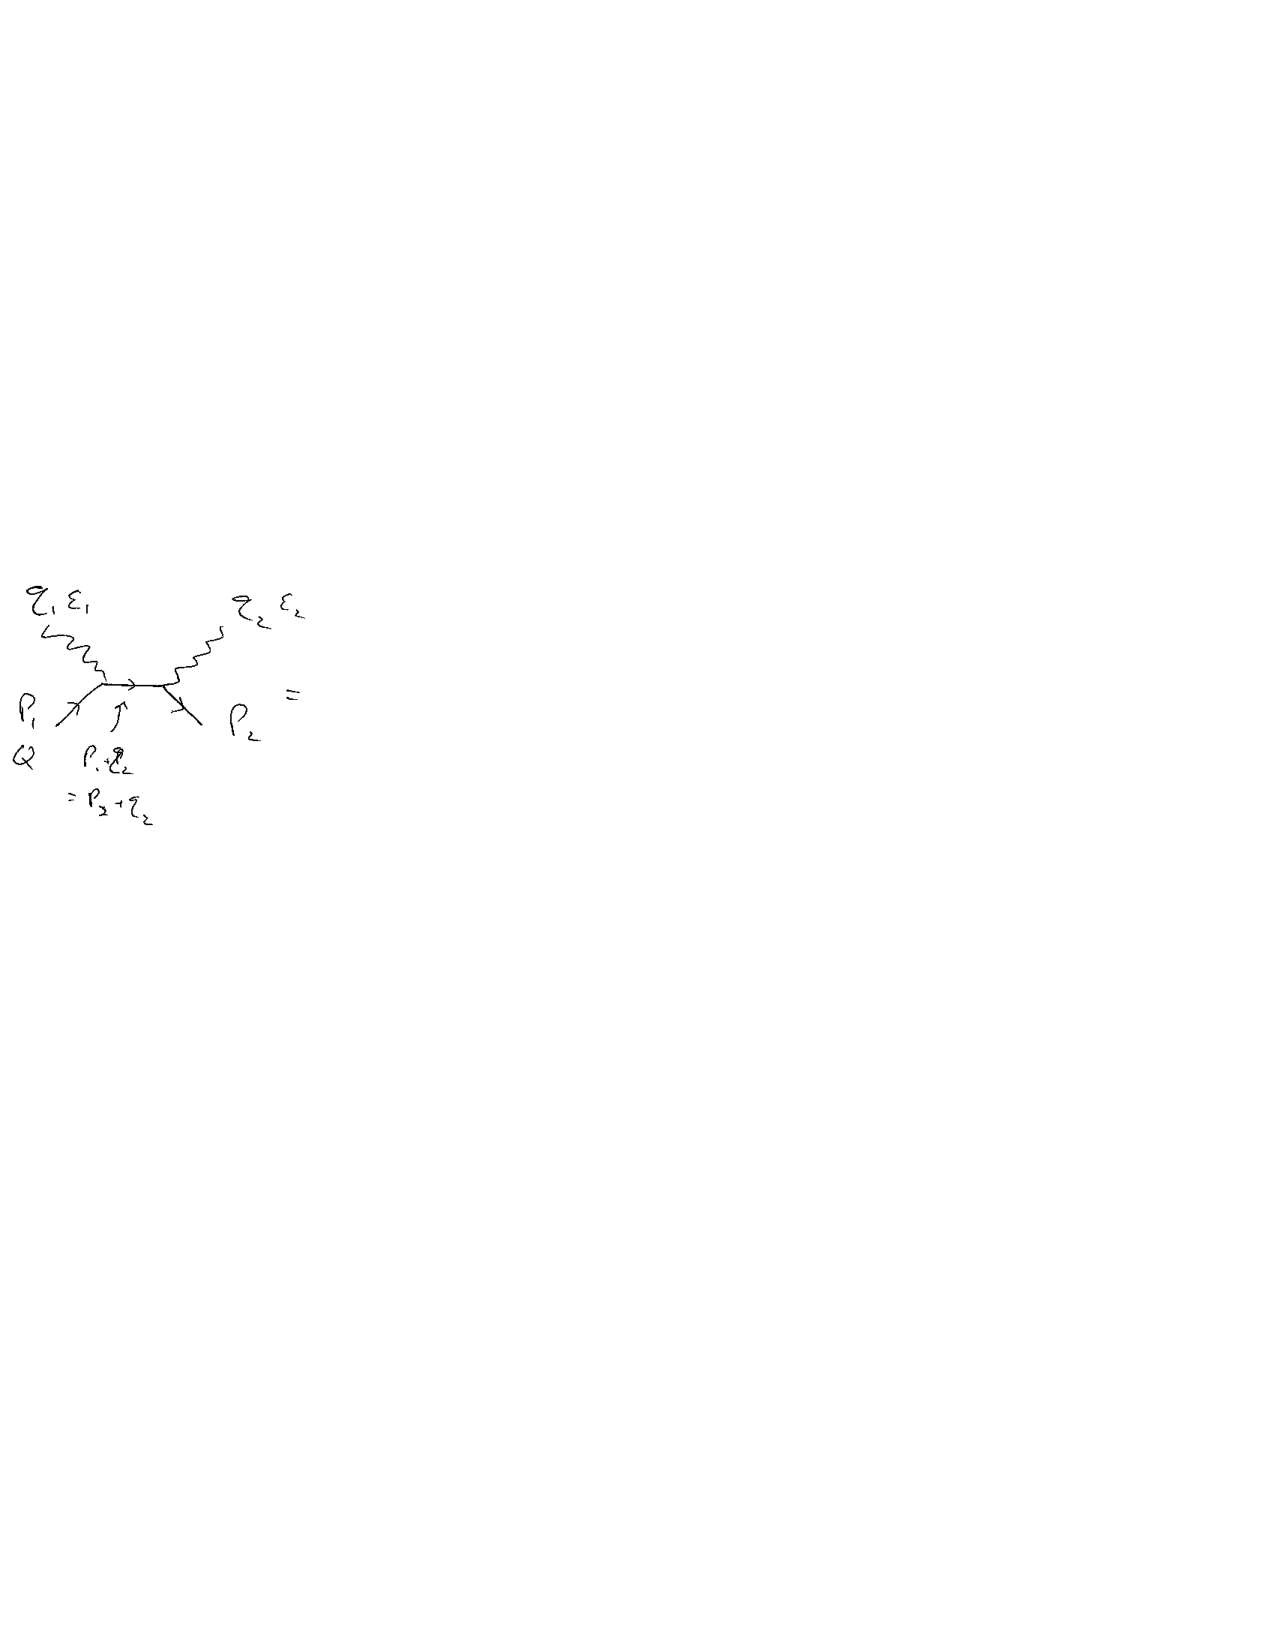
\includegraphics[width=0.9\textwidth]{./comptonScattering.pdf}
\end{minipage} %\hfill
\begin{minipage}{0.45\textwidth}
\bea
&=& (iQ)\epsilon^1_\mu(2 p_1^\mu) \frac{i}{(p_1+q_1)^2 - m^2} (iQ)\epsilon^2_\nu (2p_2^\nu)\\
&=& (-iQ^2) 4 \frac{(p_1\cdot\epsilon^1) (p_2\cdot\epsilon^2)}{m^2 + 2 p_1\cdot q_1 -m^2 }  = \epsilon_1^\mu \epsilon_2^\nu \underbrace{\left( \frac{(-iQ^2) 2 {p_1}_\mu {p_2}_\nu}{p_1\cdot q_1} \right)}_{M_{\mu\nu}}
\eea
\end{minipage}

As we said above, Lorentz Invariant $\Rightarrow q_1^\mu q_2^\nu M_{\mu\nu} = 0$\\

But here, $ q_1^\mu q_2^\nu M_{\mu\nu} = (-iQ^2) 2 (p_2\cdot q_2) \ne 0$ !

Looks like we're dead...


\clearpage

However we are forgetting a diagram.

\begin{minipage}{0.4\textwidth}
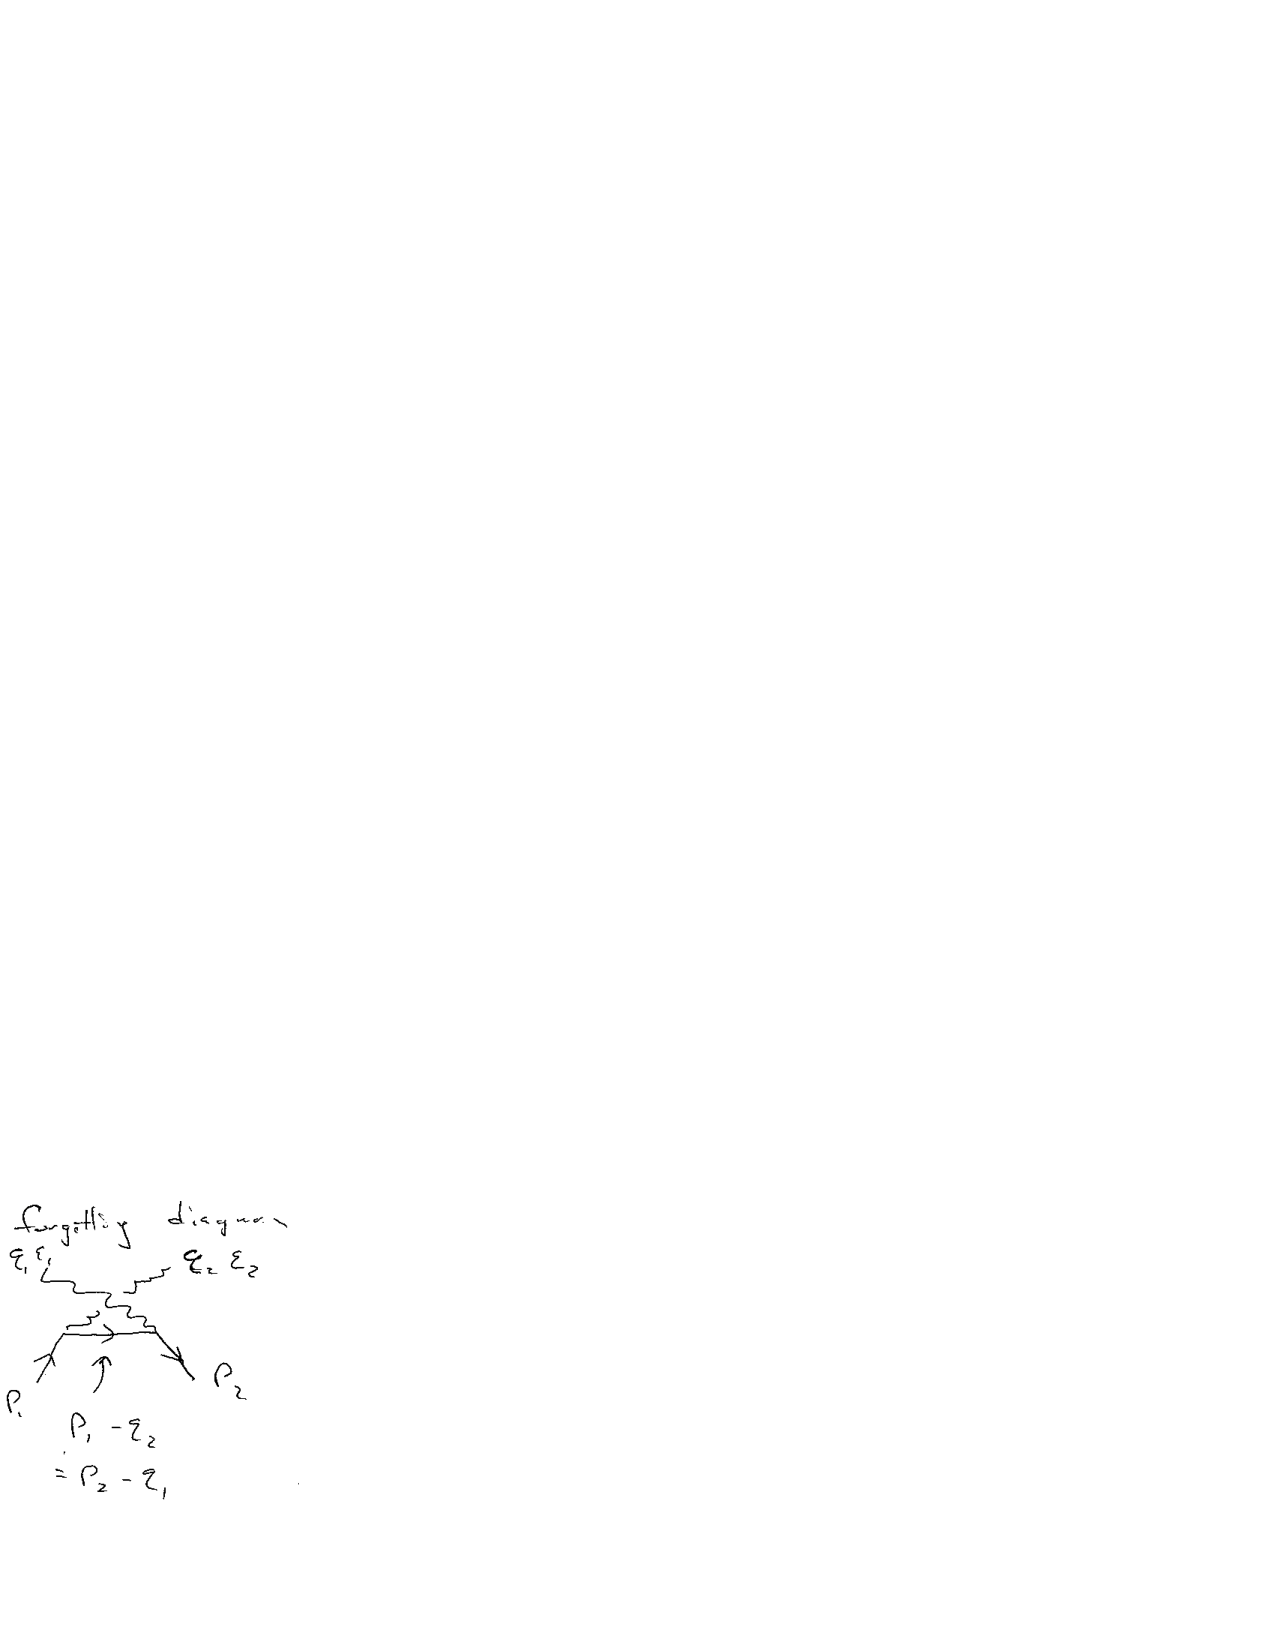
\includegraphics[width=0.9\textwidth]{./comptonScattering2.pdf}
\end{minipage}
\begin{minipage}{0.5\textwidth}
\bea
&=& (iQ)\epsilon^1_\mu(2 p_2^\mu) \frac{i}{(p_2-q_1)^2 - m^2} (iQ)\epsilon^2_\nu (2p_1^\nu)\\
&=&  \epsilon_1^\mu \epsilon_2^\nu \left( \frac{(-iQ^2) 4 {p_2}_\mu {p_1}_\nu}{-2 p_2\cdot q_1} \right) \\ 
&\underbrace{\sim}_{\textrm{Soft limit $p_1 = p_2$}}& \epsilon_1^\mu \epsilon_2^\nu \left( \frac{-(-iQ^2) 2 {p_1}_\mu {p_2}_\nu}{ p_1\cdot q_1} \right) 
\eea
\end{minipage}

and for this diagram, $ q_1^\mu q_2^\nu M_{\mu\nu} = -(-iQ^2) 2 (p_2\cdot q_2)$

So the sum $M_{\mu\nu}^A + M_{\mu\nu}^B$ is Lorentz Invariant. (Residual non Lorentz Invariant pieces of each diagram cancel)

Very good!

\lineacross 

\clearpage

Now lets do the same thing as before, but with many different possible matter particles. 

$i = 1, ... N_{\textrm{matter}}$

\begin{minipage}{0.4\textwidth}
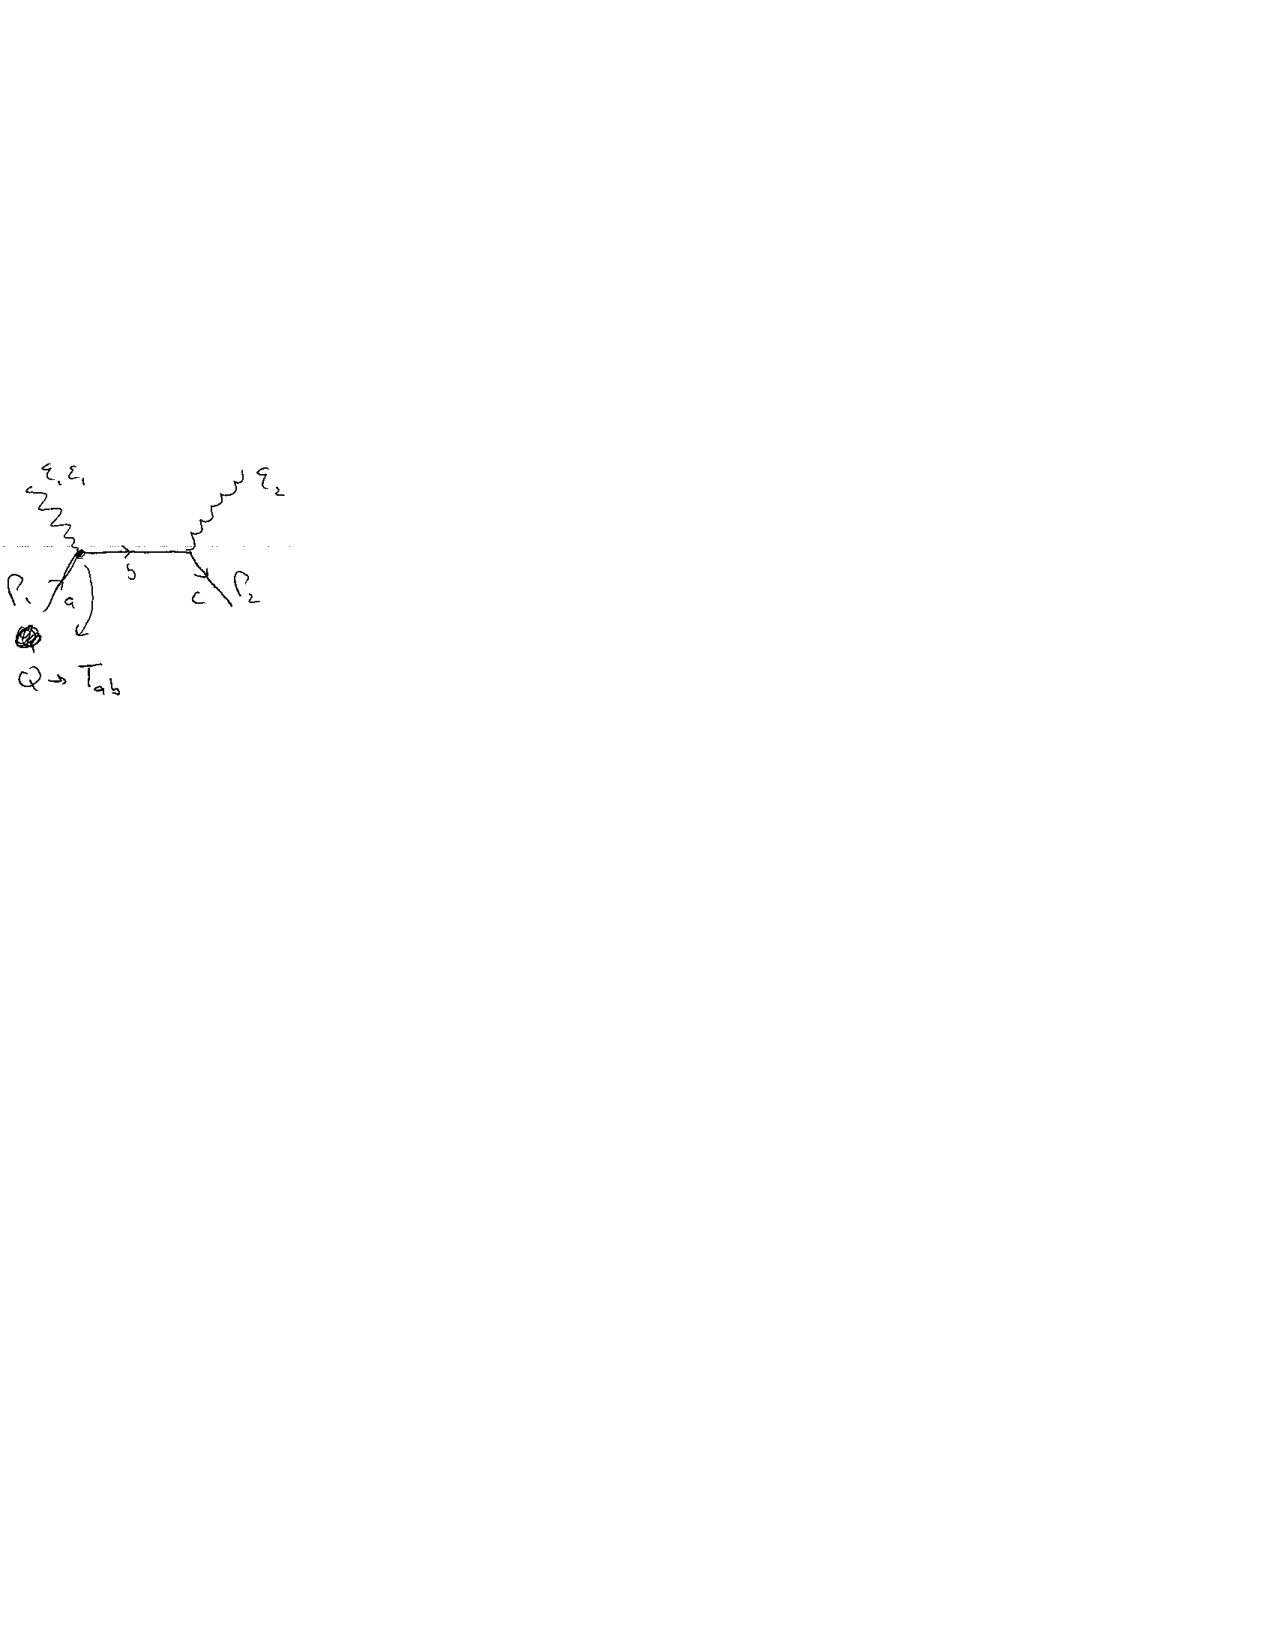
\includegraphics[width=0.9\textwidth]{./comptonScattering3.pdf}
\end{minipage}
\begin{minipage}{0.45\textwidth}
\bea
&=& (iT_{ab})\epsilon^1_\mu(2 p_1^\mu) \frac{i}{\underbrace{(p_1+q_1)^2 - m^2}_{ m_a^2 +2p_1\cdot q_1 - m_b^2}} (iT_{bc})\epsilon^2_\nu (2p_2^\nu)\\
&=&  \epsilon_1^\mu \epsilon_2^\nu \left( \frac{(-iT_{ab}T_{bc}) 4 {p_1}_\mu {p_2}_\nu}{m_a^2 +2p_1\cdot q_1 - m_b^2} \right) \equiv M^{\mu\nu}_A
\eea
\end{minipage}


Other diagram:

\begin{minipage}{0.4\textwidth}
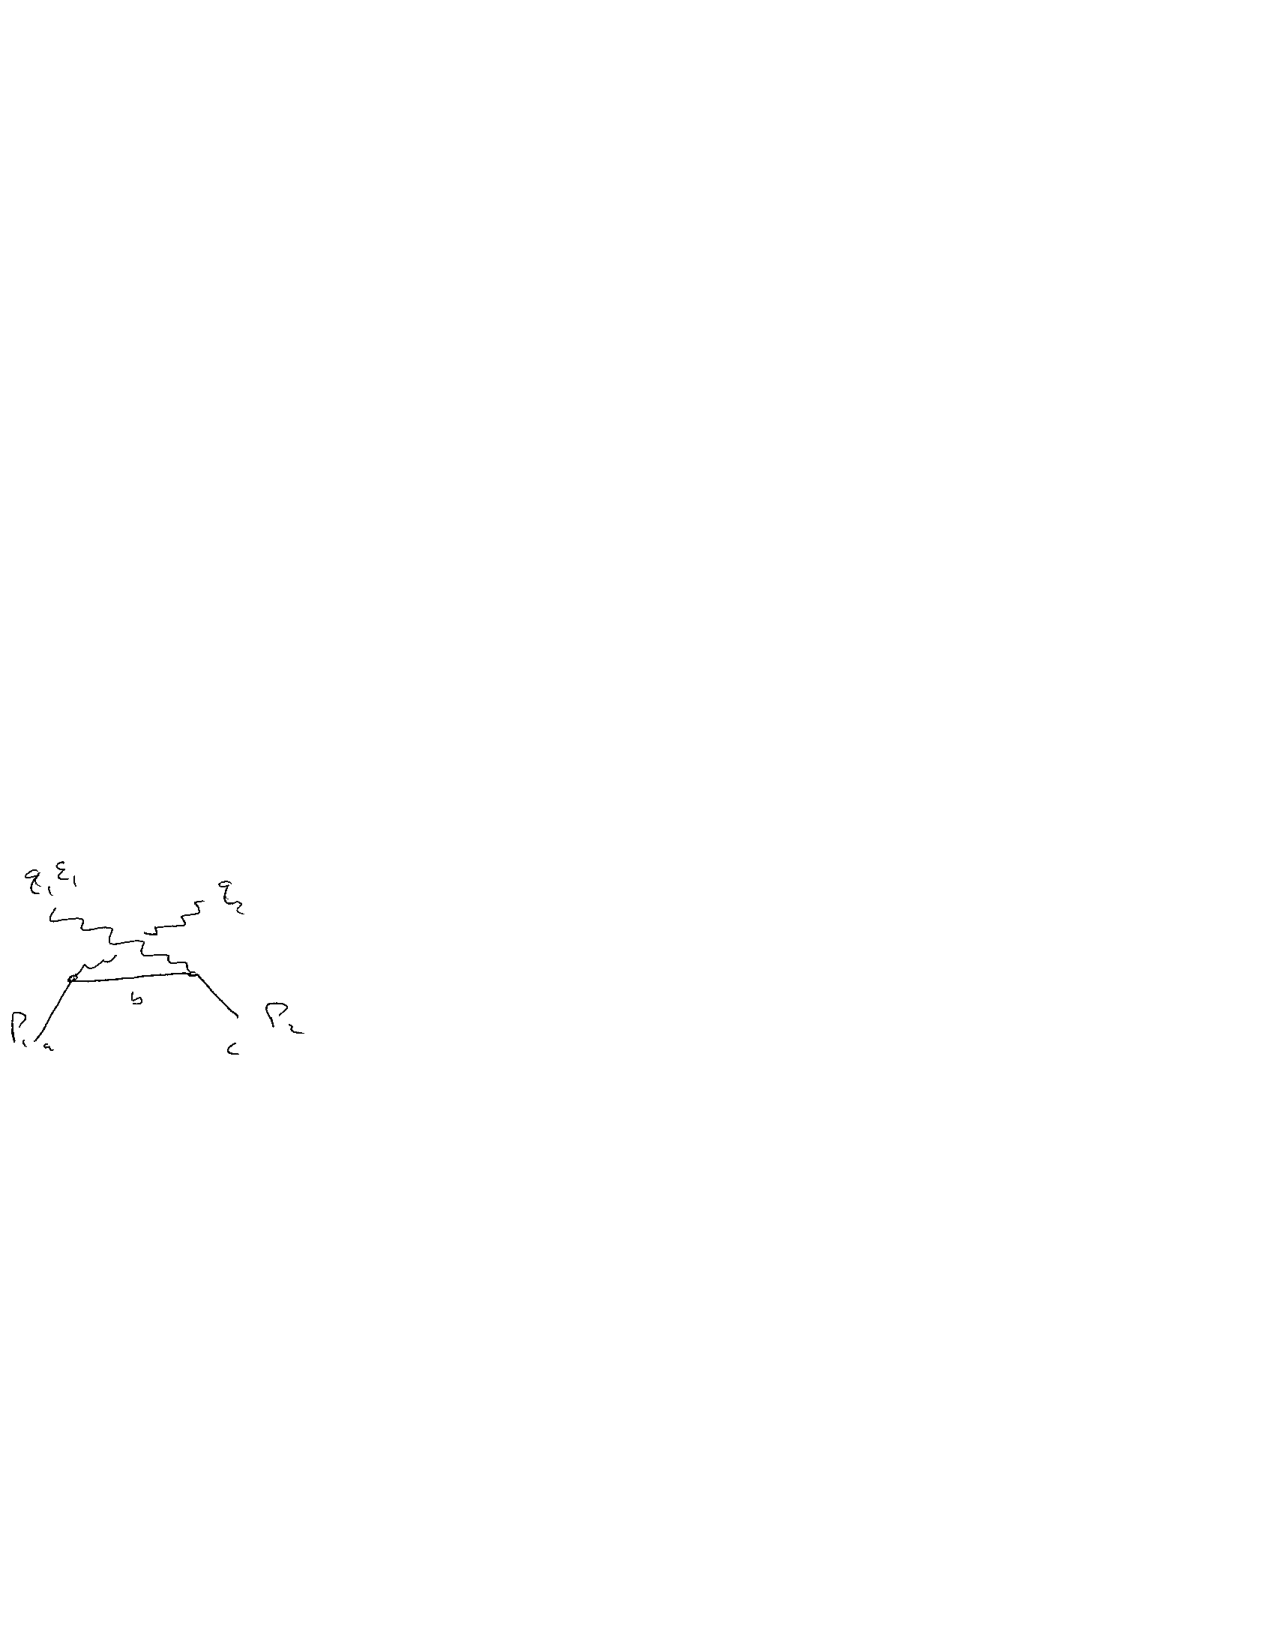
\includegraphics[width=0.9\textwidth]{./comptonScattering4.pdf}
\end{minipage} %\hfill
\begin{minipage}{0.45\textwidth}
\bea
&=&  \epsilon_1^\mu \epsilon_2^\nu \left( \frac{(-iT_{ab}T_{bc}) 4 {p_2}_\mu {p_1}_\nu}{m_a^2 - 2p_2\cdot q_1 - m_b^2} \right) \equiv M^{\mu\nu}_B 
\eea
\end{minipage} 

Now, if $m_a = m_b = m_c$ then, $ {q_1}_\mu {q_2}_\nu (M^{\mu\nu}_A + M^{\mu\nu}_B) = 0 $ as above \multiline{$m_a^2 - m_b^2 = 0$ \\ relative - size}

However if $m_a \ne m_b$, in soft limit

$ {q_1}_\mu {q_2}_\nu (M^{\mu\nu}_A + M^{\mu\nu}_B) = -\left[ \frac{(-iT_{ab}T_{bc})4}{m_a^2 - m_b^2}  (2 p_1^\mu p_1^\nu) \right] \ne 0$

{\Large Mass-less spin-1 particles can only interact with particles of the same mass!}

\lineacross

\clearpage

Now allow many different \multiline{matter fields \\ (but same mass!)} and many force carriers ``gluons'' 

$i = 1, ... N_{\textrm{matter}}$

$I = 1, ... N_{\textrm{gluons}}$

\begin{minipage}{0.4\textwidth}
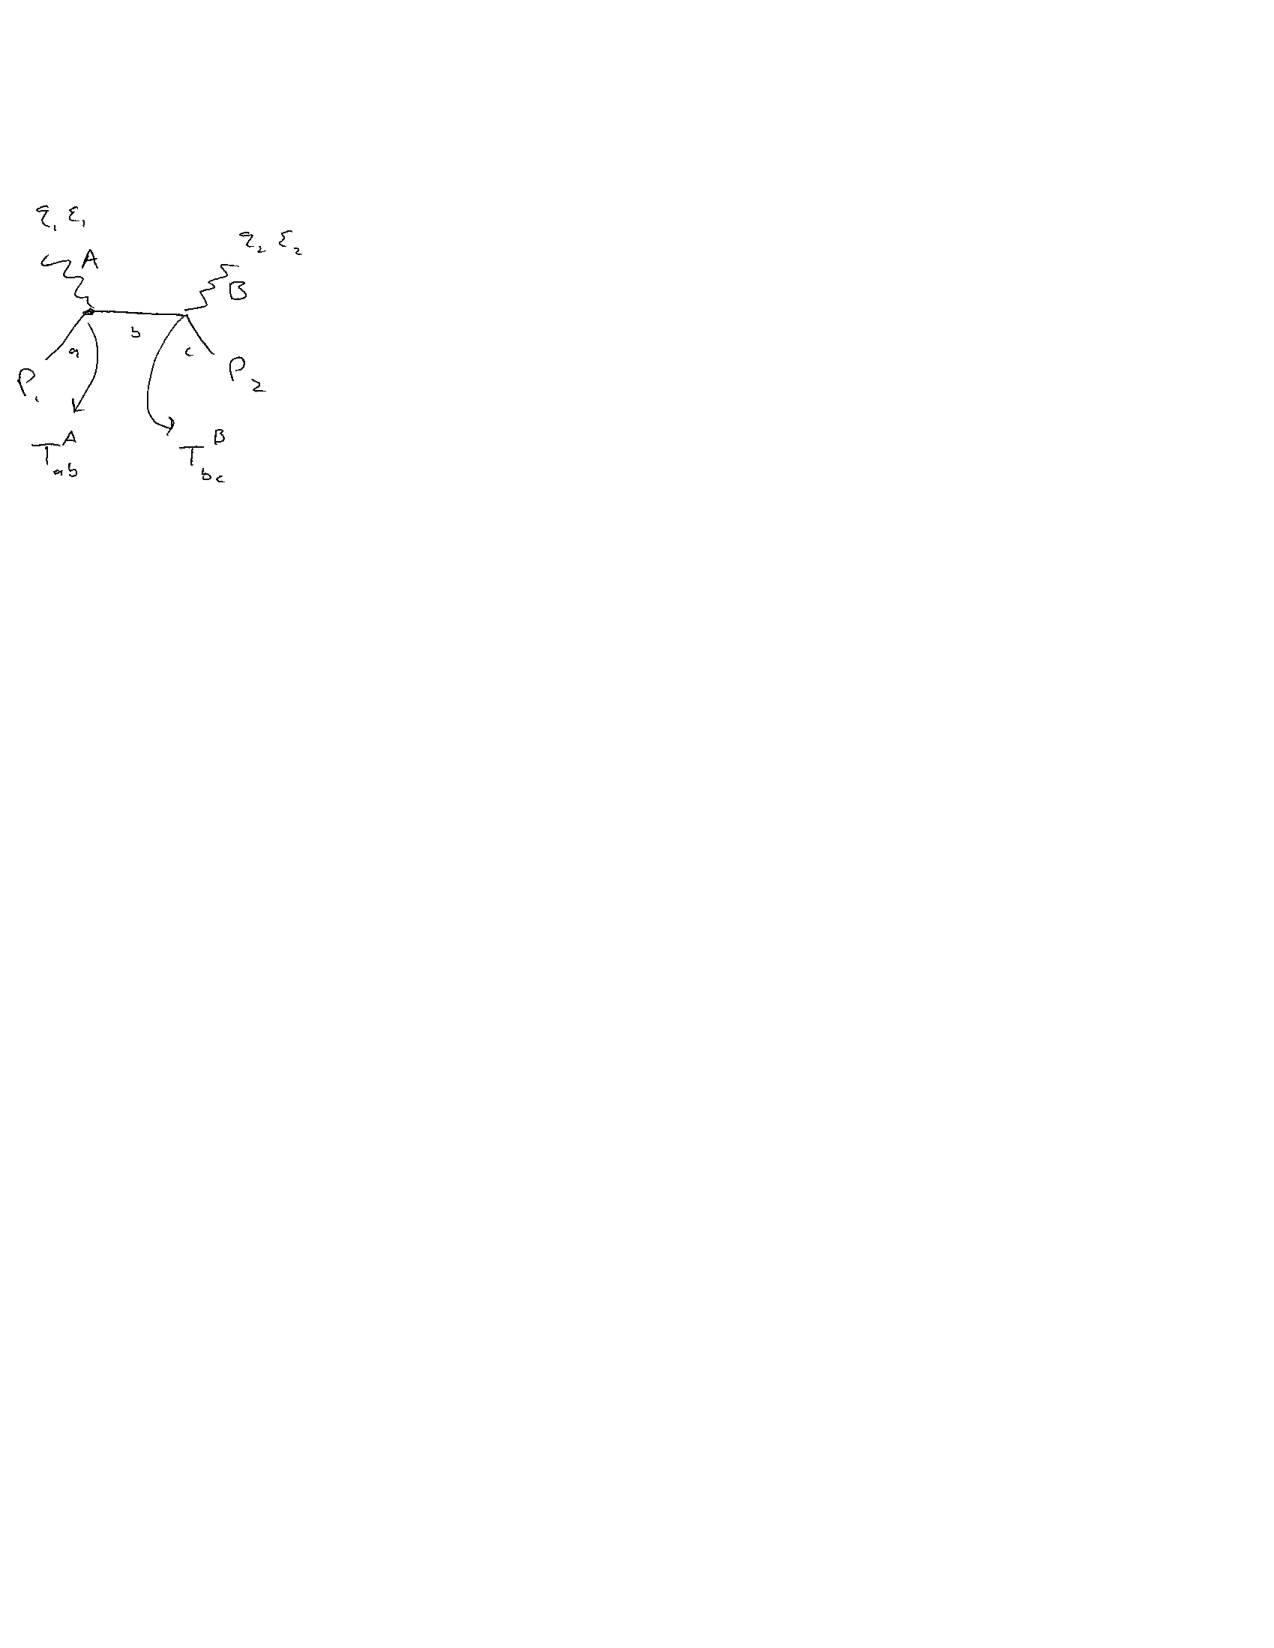
\includegraphics[width=0.9\textwidth]{./comptonScattering5.pdf}
\end{minipage} %\hfill
\begin{minipage}{0.45\textwidth}
\bea
&=&  \epsilon_1^\mu \epsilon_2^\nu \left( \frac{(-iT_{ab}^AT_{bc}^B) 4 {p_1}_\mu {p_2}_\nu}{2p_1\cdot q_1 } \right) \equiv M^{\mu\nu}_A
\eea
\end{minipage} %\hfill

and 


\begin{minipage}{0.4\textwidth}
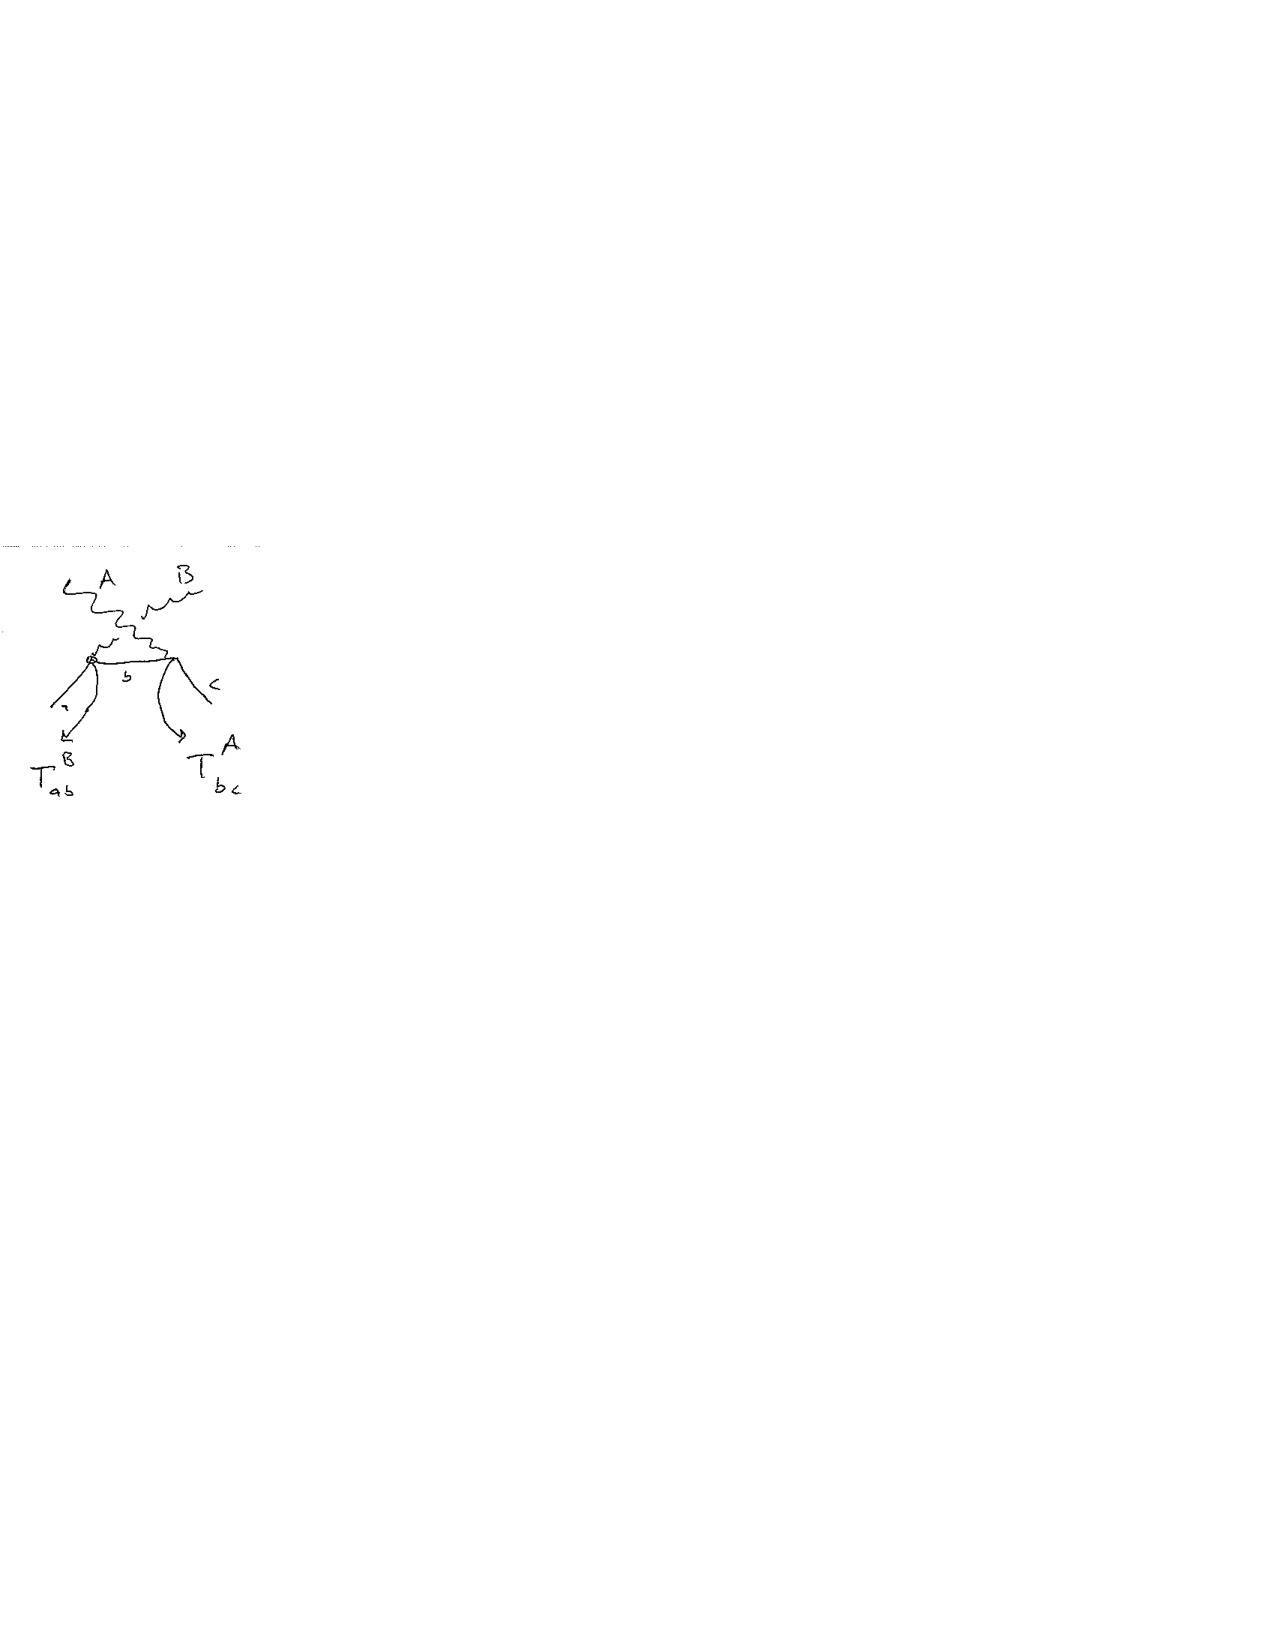
\includegraphics[width=0.9\textwidth]{./comptonScattering6.pdf}
\end{minipage} %\hfill
\begin{minipage}{0.45\textwidth}
\bea
&\underbrace{=}_{\textrm{``soft limit''}}&  \epsilon_1^\mu \epsilon_2^\nu \left( \frac{(-iT_{ab}^BT_{bc}^A) 4 {p_1}_\mu {p_2}_\nu}{- 2p_1\cdot q_1 } \right) \equiv M^{\mu\nu}_B
\eea
\end{minipage} %\hfill

Now, 

\bea
 {q_1}_\mu {q_2}_\nu (M^{\mu\nu}_A + M^{\mu\nu}_B) &=& 2(-i)(p_2\cdot q_2)(T_{ab}^AT_{bc}^B - T_{ab}^BT_{bc}^A) \\ 
&=& 2(-i)(p_2\cdot q_2) [T^A, T^B]
\eea
$[T^A, T^B]$ not 0 for random Ts. 

In fact, another diagram we are missing:

\begin{minipage}{0.4\textwidth}
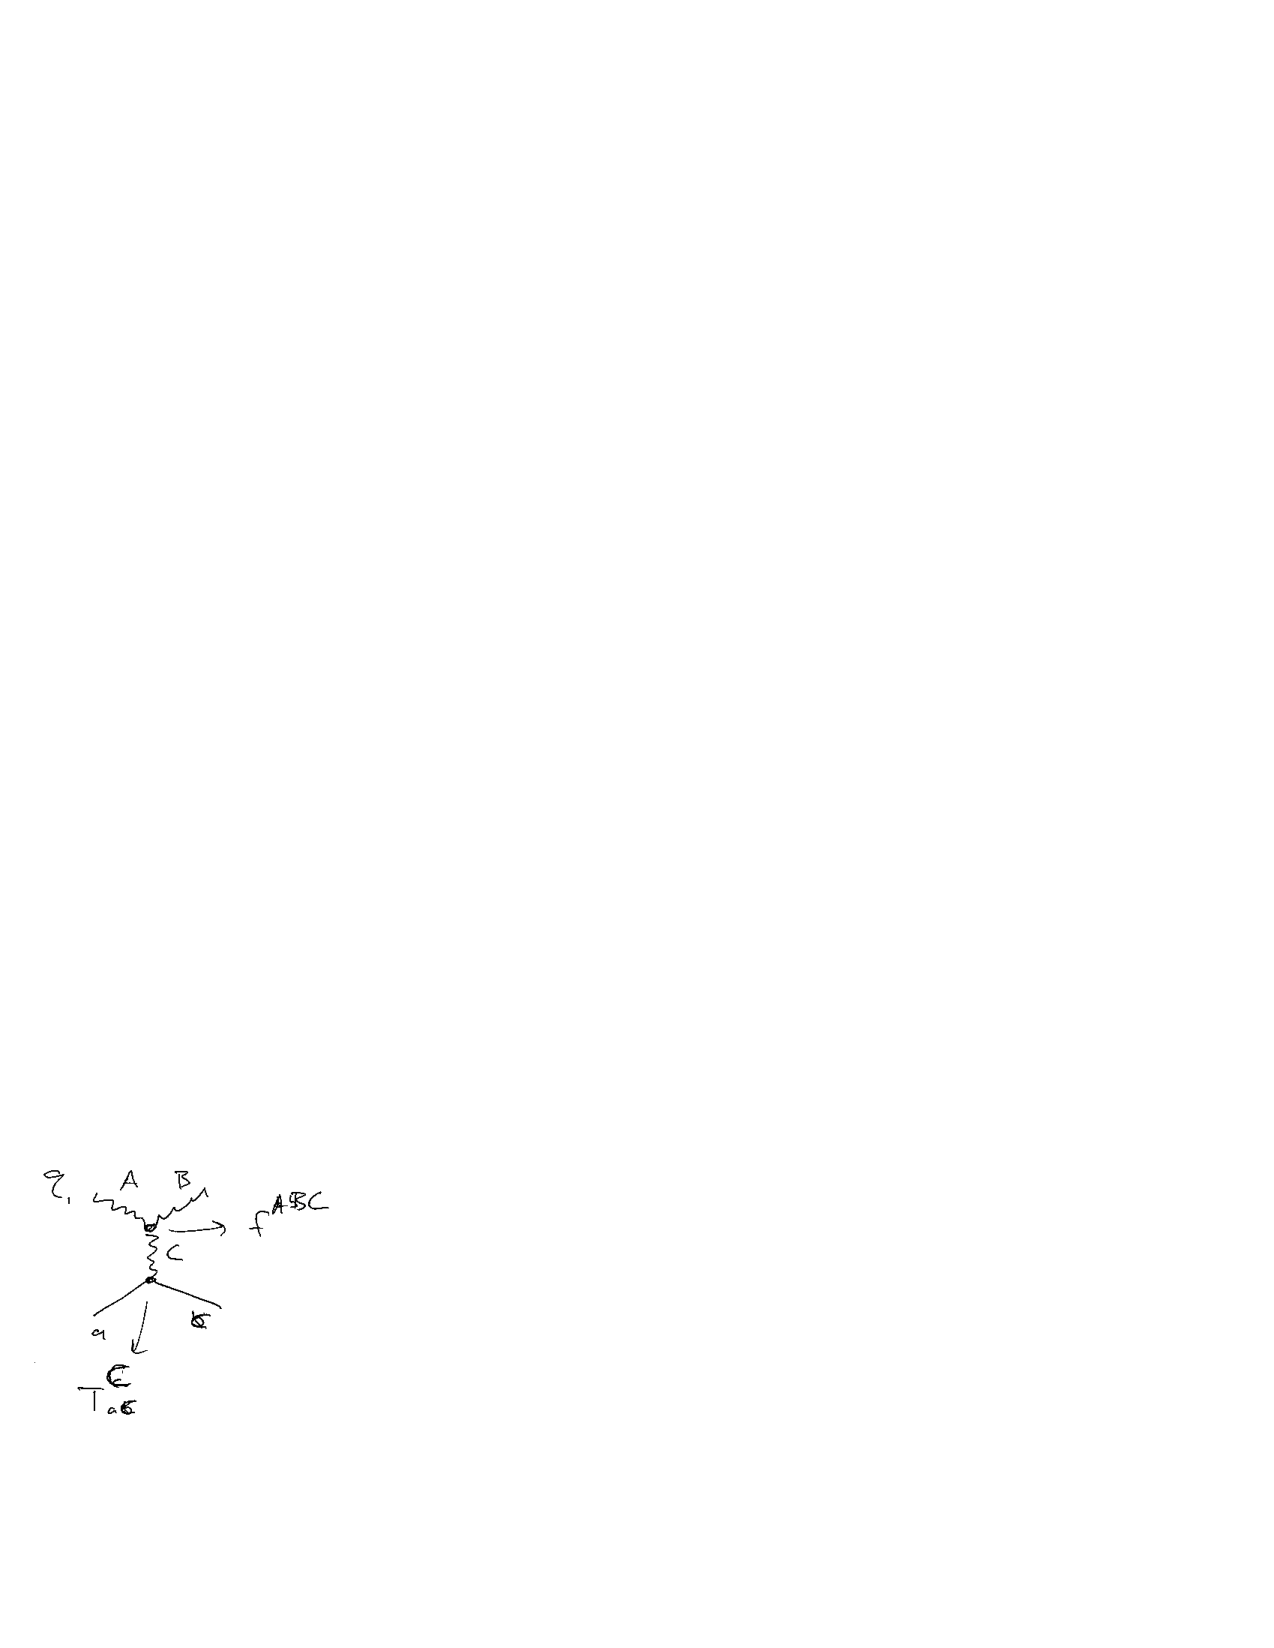
\includegraphics[width=0.9\textwidth]{./comptonScattering7.pdf}
\end{minipage} %\hfill
\begin{minipage}{0.45\textwidth}
\be
= + 2i (q\cdot q) i f^{ABC} T_{ac}^C 
\ee
\end{minipage} %\hfill

Sum of all three only Lorentz invariant if 

\be
[T^A, T^B] = i f^{ABC} T^C
\ee


``gluons'' (or any other group of interacting mass-less spin-1 particles) must transform as a Lie group ! 

Only question is which group, there are only a finite handful of possibilities


``Yang-Mills'' Interaction. 

\lineacross


\underline{Now do the same thing to a more general interaction}


\begin{figure}[h]
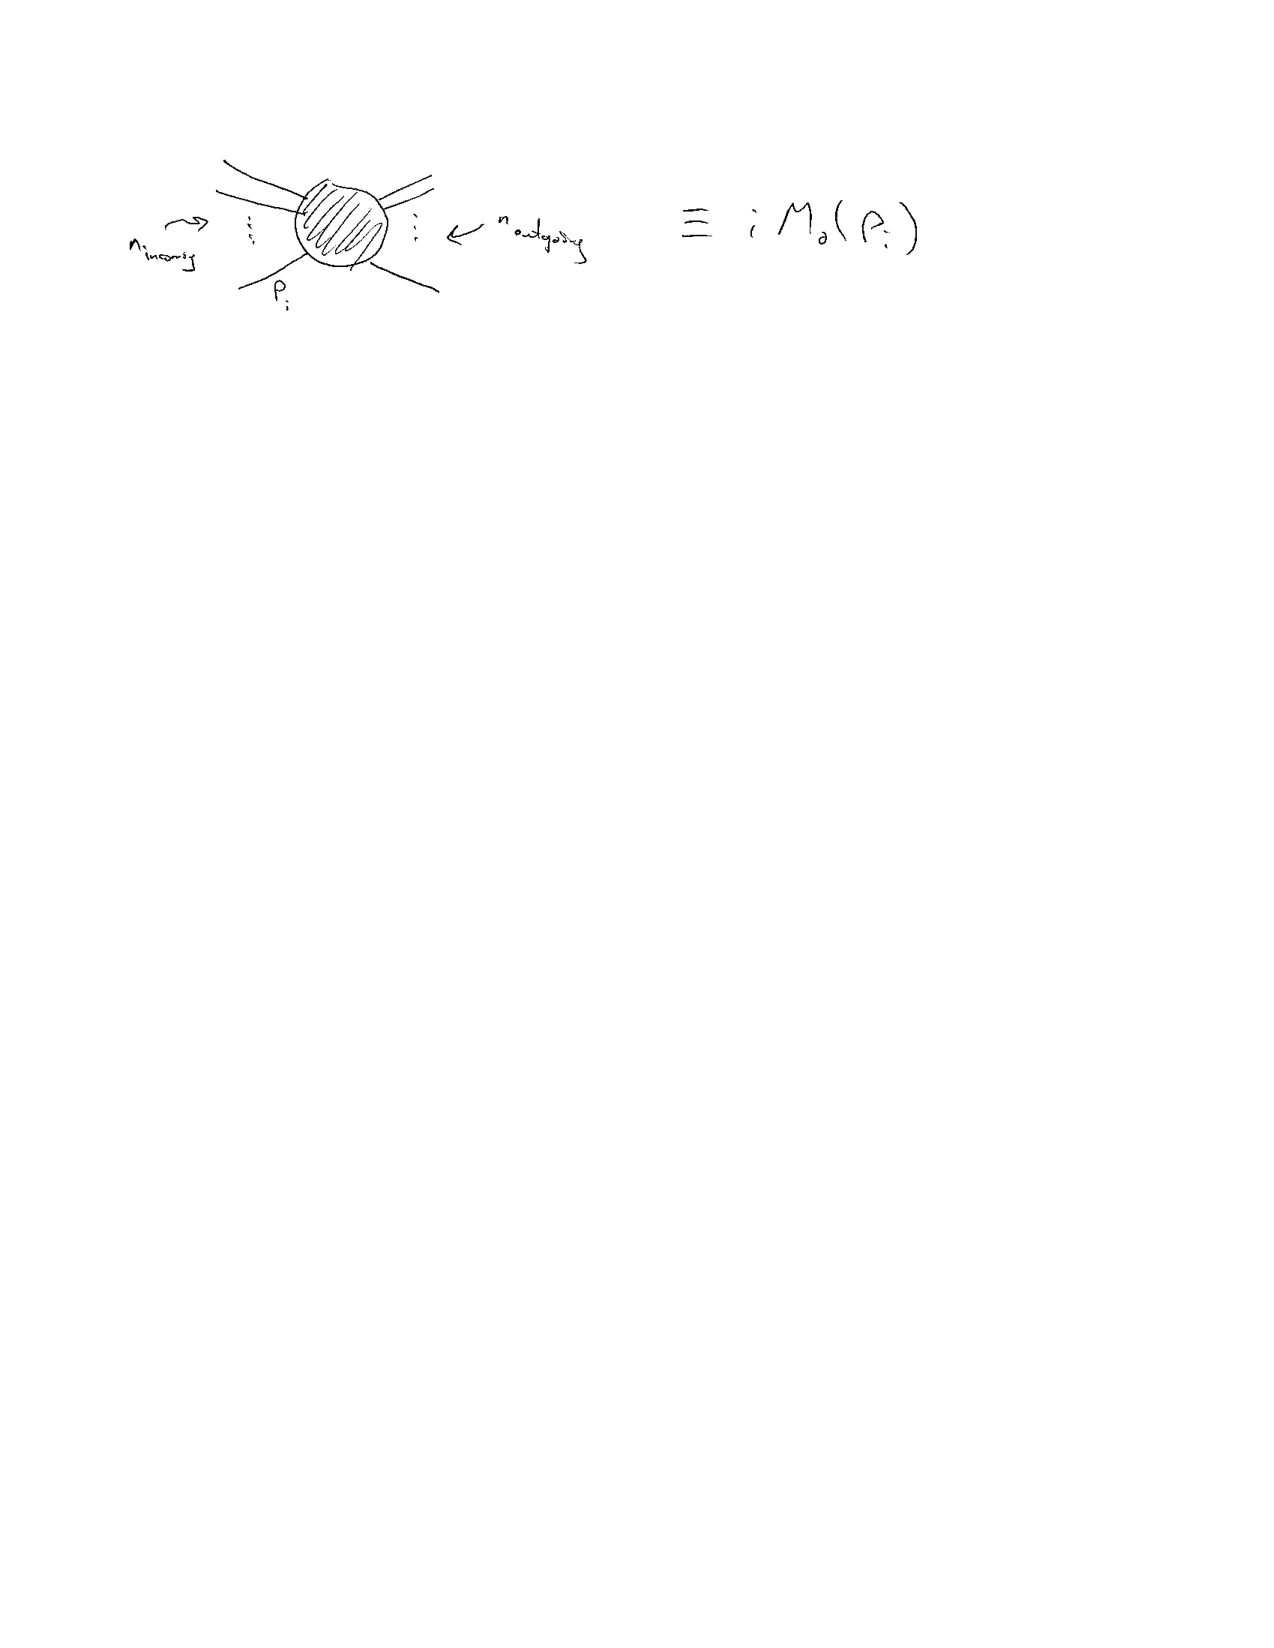
\includegraphics[width=0.99\textwidth]{./generalScattering.pdf}
\end{figure}

Consider what happens if we attach a ``photon'' to an incoming leg

\begin{figure}[h]
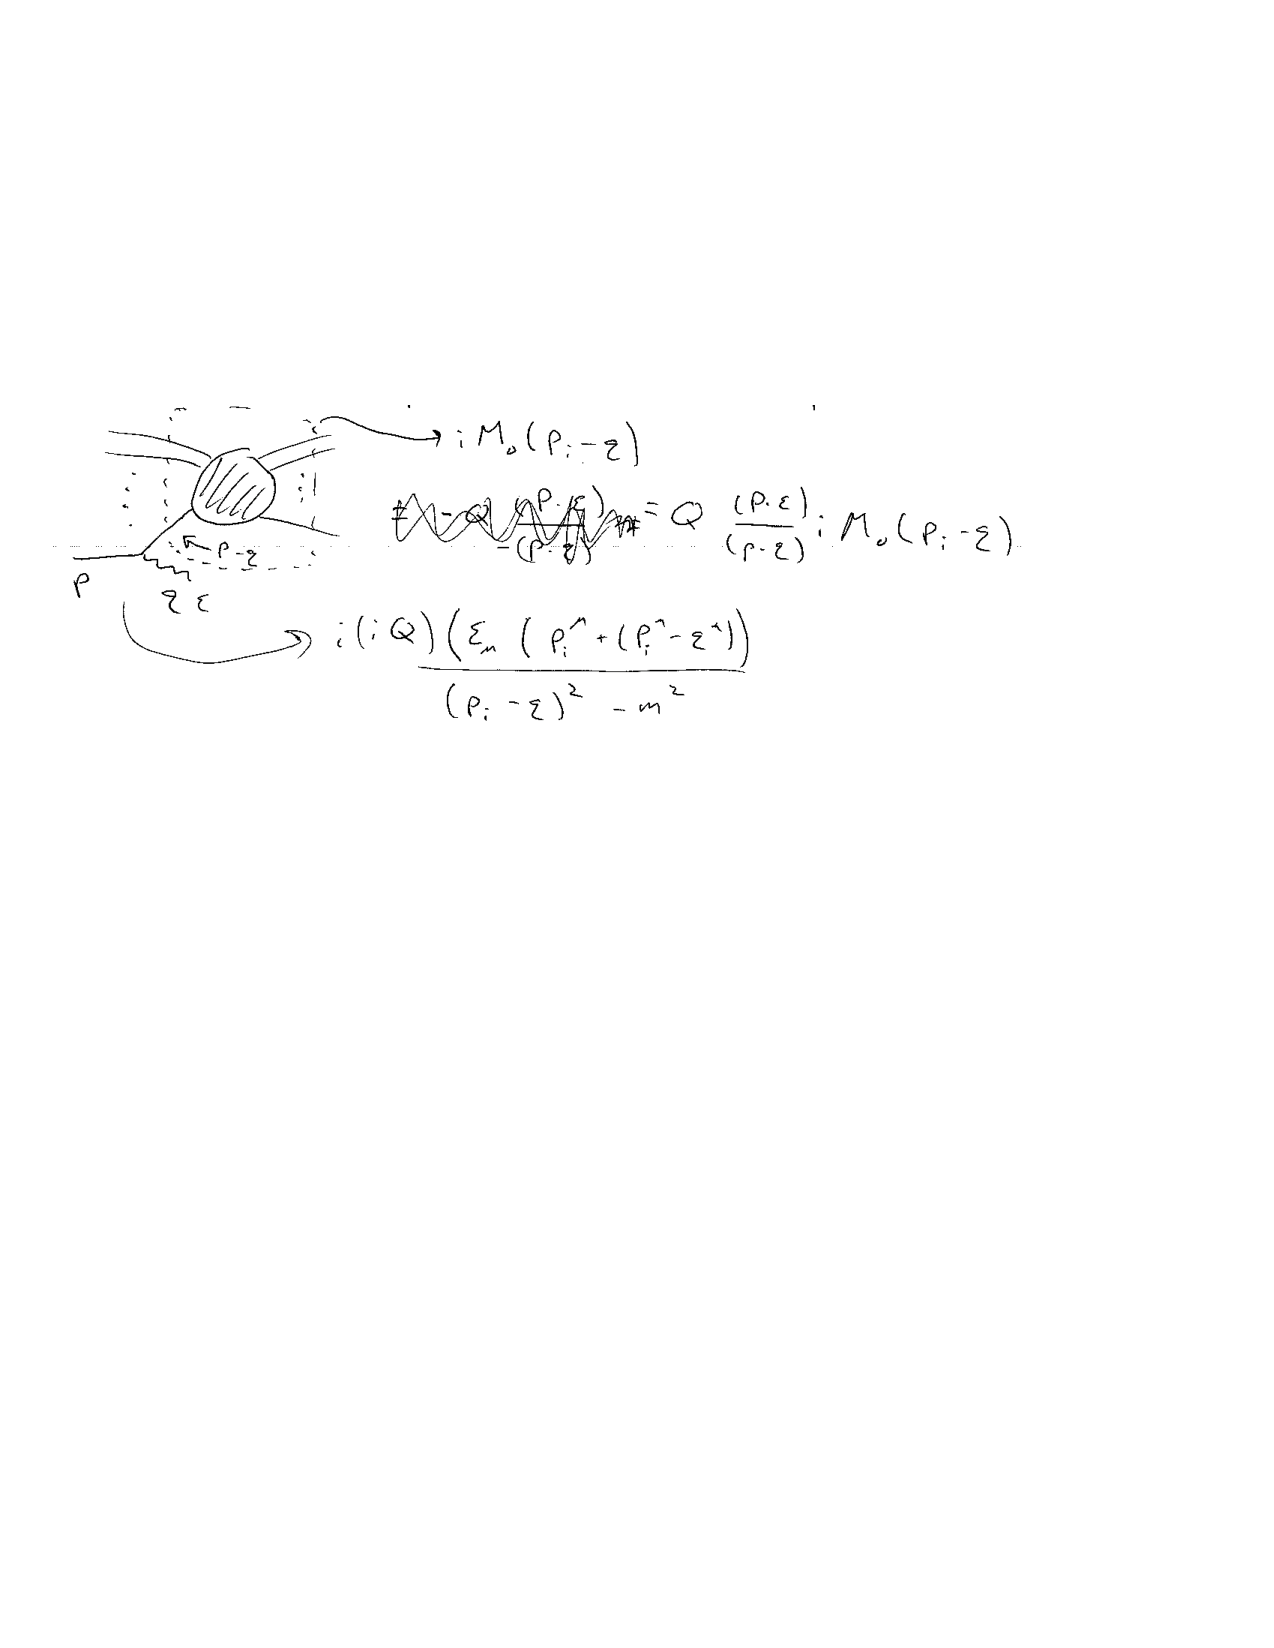
\includegraphics[width=0.99\textwidth]{./incomingPhoton.pdf}
\end{figure}

\clearpage

Can also attach photon to outgoing leg

\begin{figure}[h]
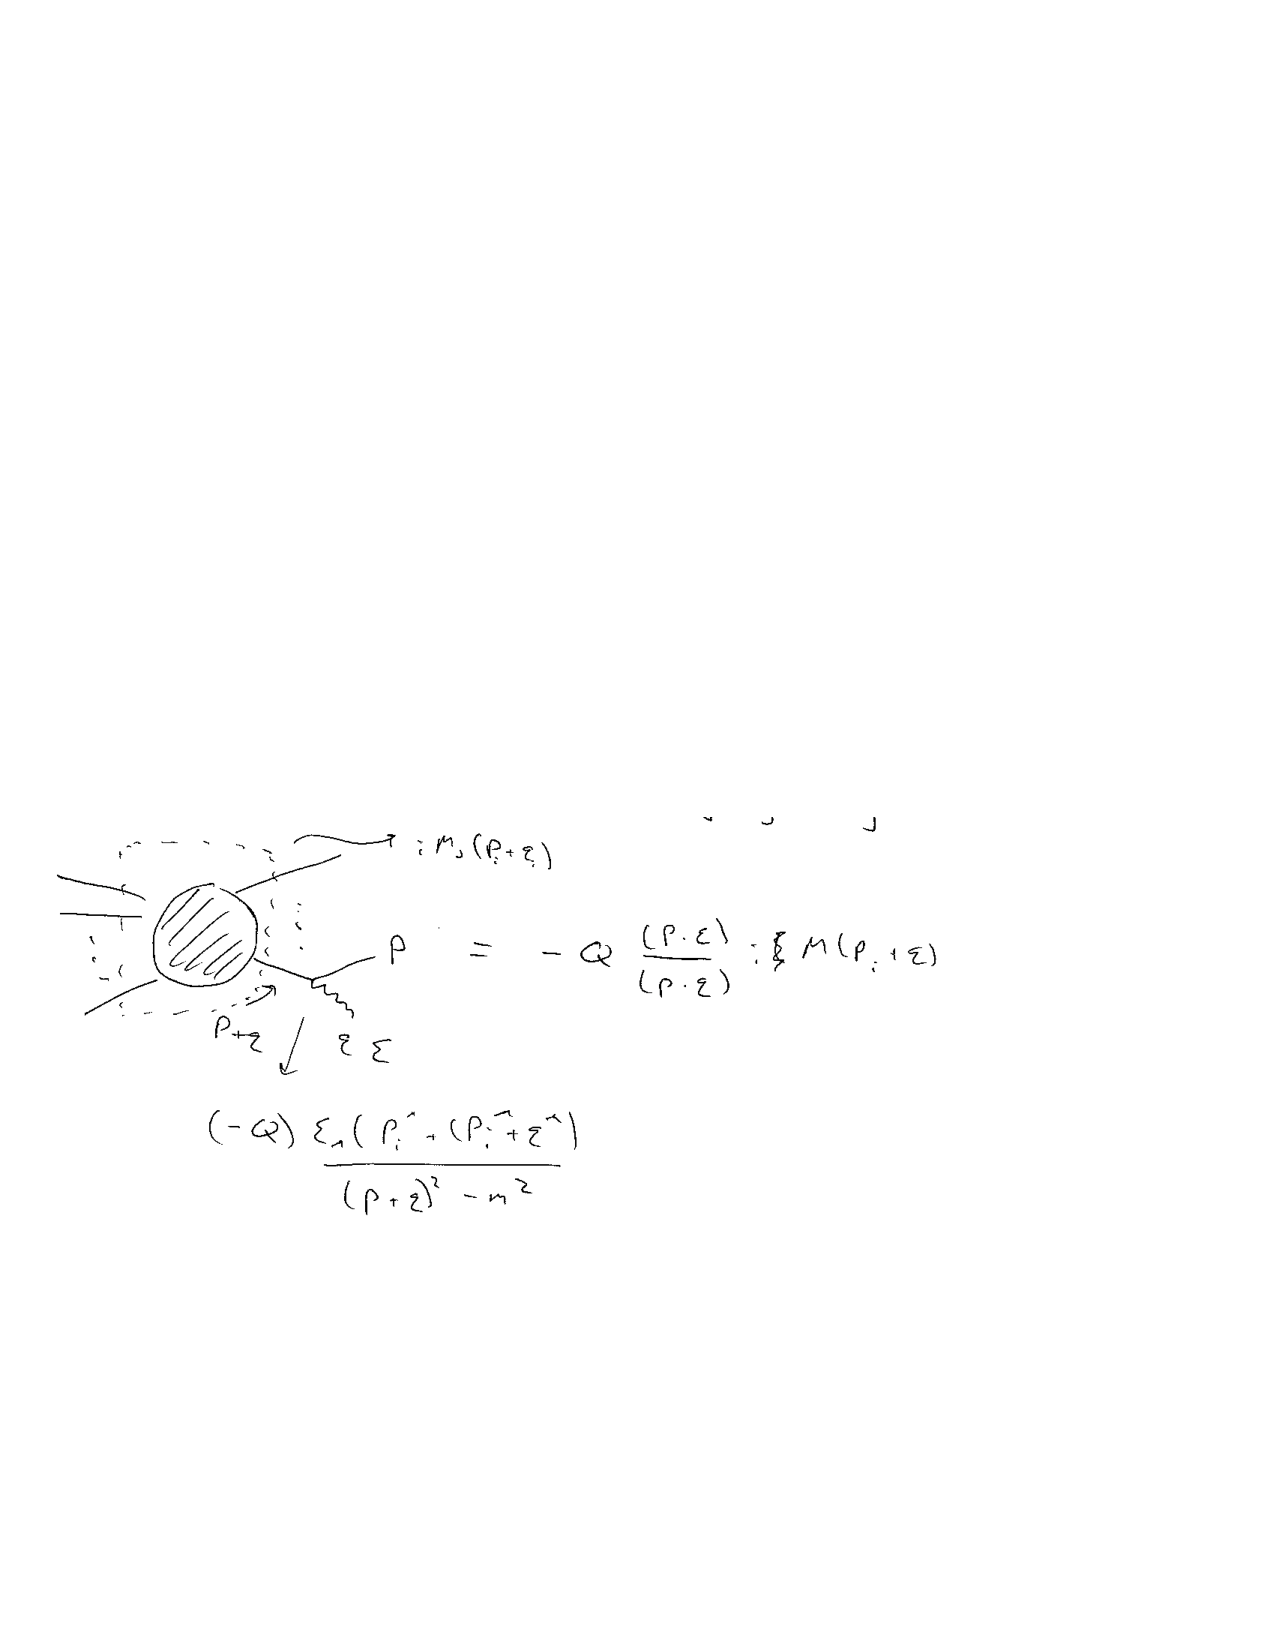
\includegraphics[width=0.99\textwidth]{./outgoingPhoton.pdf}
\end{figure}

Total Amplitude is then given by

\be
M  = \sum_{\rmt{incoming}} Q_i \frac{(p\cdot\epsilon)}{(p\cdot q)}\ i M_0(p-q) + \sum_{\rmt{outgoing}} - Q_i \frac{(p\cdot\epsilon)}{(p\cdot q)}\ i M_0(p+q)
\ee

Take soft limit: $M_0(p\pm q) \rightarrow M_0(p)$

\be
M  = iM_0 \left( \sum_{\rmt{incoming}} Q_i \frac{(p\cdot\epsilon)}{(p\cdot q)}\  + \sum_{\rmt{outgoing}} - Q_i \frac{(p\cdot\epsilon)}{(p\cdot q)}\   \right)
\ee

Now as before $\epsilon_\mu \rightarrow \epsilon'_\mu + q_\mu$ means that M must vanish when $\epsilon_\mu \rightarrow q_\mu$.

OR under a Lorentz Transform

\be
\epsilon_\mu \cdot M \rightarrow \epsilon'_\mu \cdot M' + i M_0 \underbrace{\left( \sum_{\rmt{incoming}} Q_i  + \sum_{\rmt{outgoing}} - Q_i    \right)}_{\substack{= 0\ \rmt{only if} \\ \sum_{\rmt{incoming}} Q_i = \sum_{\rmt{outgoing}} Q_i }}
\ee

\underline{\underline{Charge has to be conserved! }}

\lineacross

Now same logic for Spin-2  (describes interaction w/Gravitons)

Same as above except 2-component polarization vector.


\be
\epsilon_{\mu\nu} \underbrace{\rightarrow}_{\rmt{under little group}} \epsilon_{\mu\nu} + \underbrace{A_\mu q_\nu + B_\mu q_\mu + C q_\mu q_\nu}_{\rmt{effect from all of these need to be 0 as before}}
\ee

where A, B C's are non-zero and depend on the particular little group transformation done.


\begin{minipage}{0.4\textwidth}
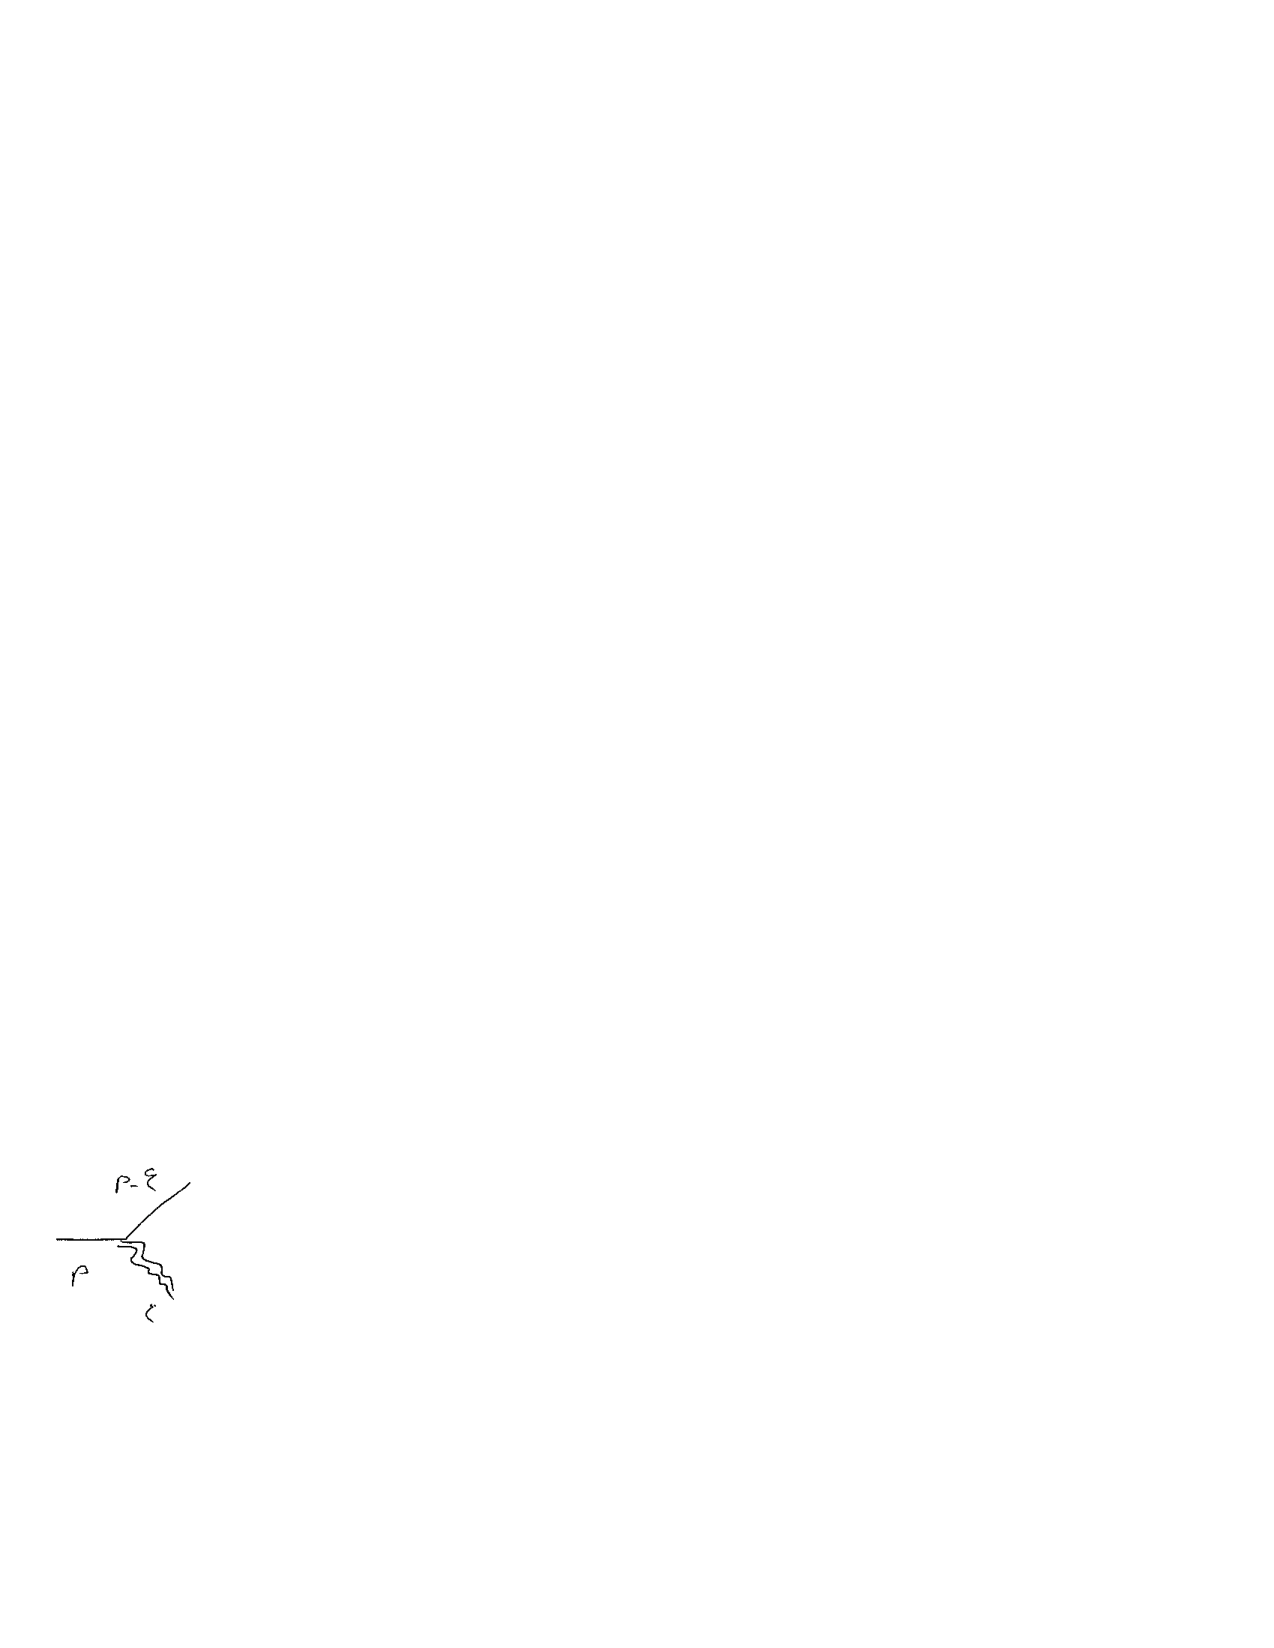
\includegraphics[width=0.9\textwidth]{./gravitonVertex.pdf}
\end{minipage} %\hfill
\begin{minipage}{0.45\textwidth}
\be
= i (iK_i) \epsilon_{\mu\nu} \frac{(p^\mu p^\nu)}{-p\cdot q}
\ee
\end{minipage} %\hfill

(Same idea with the outgoing leg)


Now, (lets focus on piece that goes like $\epsilon_{\mu\nu} \rightarrow  \epsilon_{\mu\nu}  + q_\mu B_\nu$

\bea
\epsilon_{\mu\nu} \rightarrow  \epsilon'_{\mu\nu} M'^{\mu\nu} &+& M \left( \sum_{\rmt{incoming}} K_i B_\nu p^\nu - \sum_{\rmt{outgoing}} K_i B_\nu p^\nu \right)\\
&+& M B_\nu \left( \sum_{\rmt{incoming}} K_i  p^\nu - \sum_{\rmt{outgoing}} K_i  p^\nu \right)
\eea

$\Rightarrow  K_i p_i^\nu$  is \underline{\underline{conserved}}


We know that $p_i^\nu$ is conserved by E and momentum conservation. 

Only way can have nontrivial solutions is if $k_i = k$ for all i

All particles interact with gravity with the same strength. 

\underline{Gravitational interaction is Universal !}

Discovered the ``Principle of Equivalence'' that is the starting point of General Relativity!

\lineacross

Can keep going...

For a massless spin-3 particle we would do the same exercise. 

We would find we need

\be
 \sum_{\rmt{incoming}} \beta_i  p_i^\mu p_i^\nu = \sum_{\rmt{outgoing}} \beta_i  p_i^\mu  p_i^\nu 
\ee

eg: $\mu\nu = 0$

\be
 \sum_{\rmt{incoming}} \beta_i  E_i^2 = \sum_{\rmt{outgoing}} \beta_i  E_i^2
\ee


Way too constraining.  

Only way if $\beta_i = 0$

\underline{\underline{There can be no interacting theories of massless particles of Spin greater than 2 !}}


}
\end{document}

